
\documentclass[a4paper, 12pt]{article}

\usepackage{amsmath}
\usepackage{amssymb}
\usepackage{graphicx}
\usepackage{listings}[language=C++]
\lstdefinestyle{mystyle}{
    breakatwhitespace=false,         
    breaklines=true,                 
    captionpos=b,                    
    keepspaces=true,                 
    numbers=left,                    
    numbersep=5pt,                  
    showspaces=false,                
    showstringspaces=false,
    showtabs=false,                  
    tabsize=2
}

\lstset{style=mystyle}

\title{Lab-06 Report}
\author{st122246}

\begin{document}
	
\maketitle

\section{OpenSFM}


	\begin{figure}
		\caption{Berlin Dataset}
		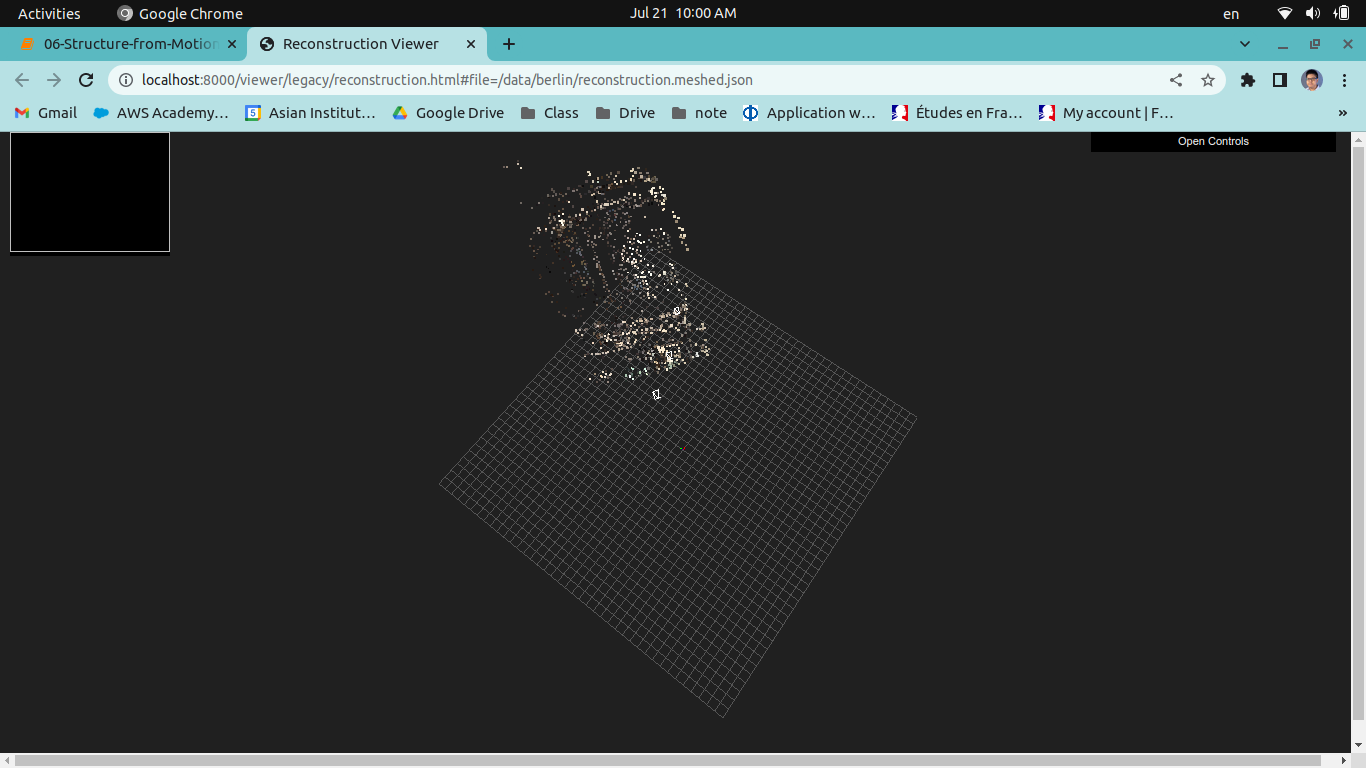
\includegraphics[scale=0.25]{images/opensfm-01.png}
	\end{figure}


	\begin{figure}
		\caption{Lab06 frames Dataset}
		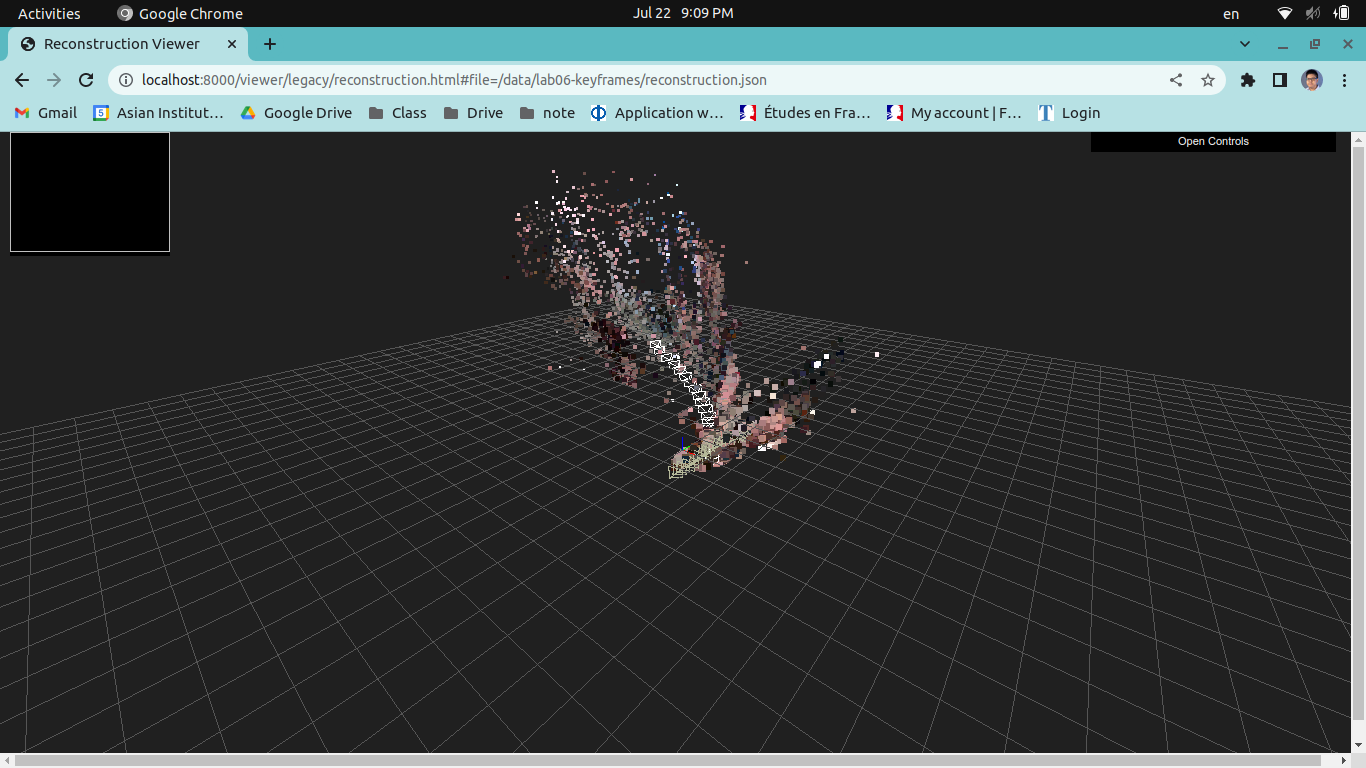
\includegraphics[scale=0.25]{images/opensfm-02.png}
	\end{figure}


	\begin{figure}
		\caption{Reconstruction of Lab06 frames Dataset}
		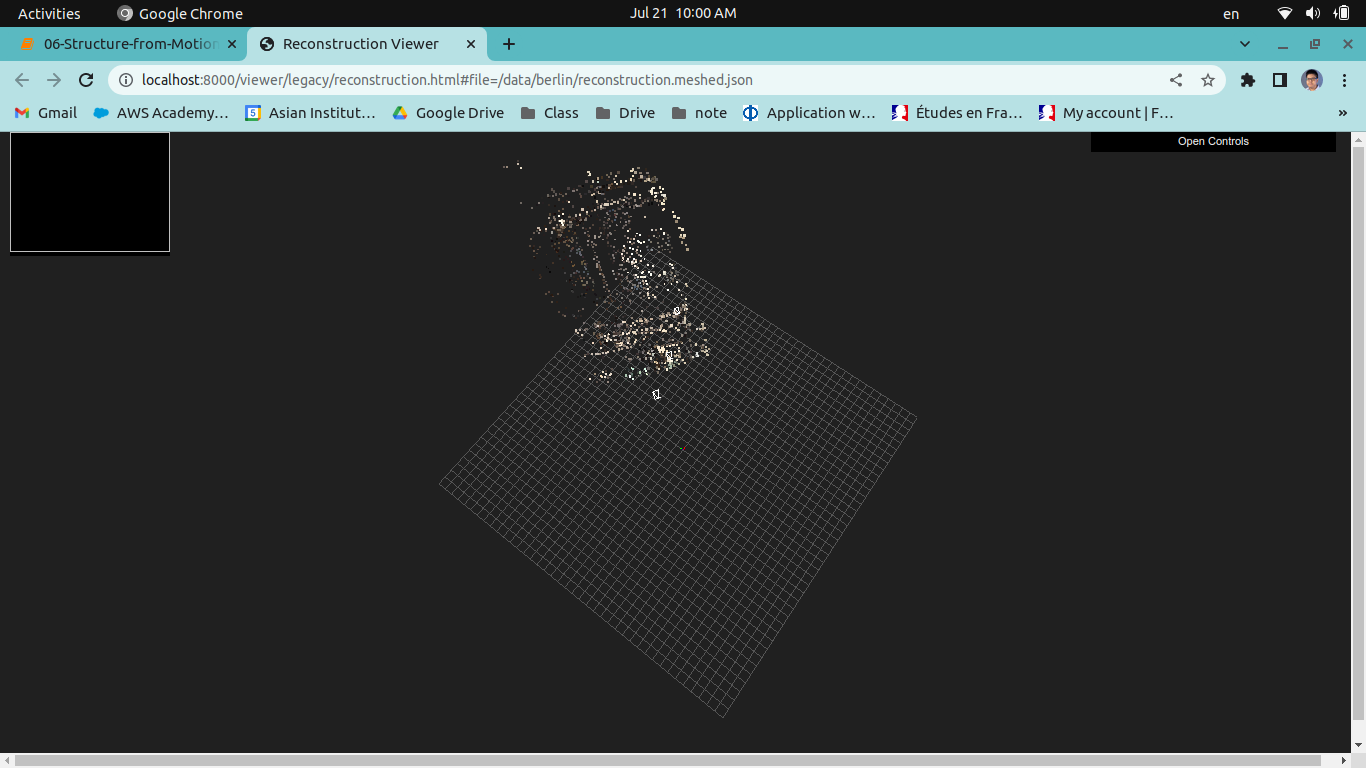
\includegraphics[scale=0.25]{images/opensfm-01.png}
	\end{figure}

	Improvement
	\begin{itemize}
		\item Q: Do you think the automatically extraced distortion parameters are working well? \\ Ans:Automatically extracted distortion parameters are not working well. Radial distortion can still be seen in undistorted images.
		\item Q: Does esitmated camera parameters seem reasonable? \\ Ans: Estimated camera parameters seems not reasonable.
		\item Q: Would giving your own parameters be better? \\ Ans: Giving own parameters improve the result.
	\end{itemize}

	Thought experiments
	\begin{itemize}
		\item 
		How could you write a program to automatically extract keyframes using optical flow method?

		The program would do the following:
		- Optical flow method calculated of each frame and selected frame with extreme optical difference as key frame and others as candidate keyframes
		- By calculating the mutual information of key frame set,  the minimum mutual information entropy is taken as threshold
		- Frame larger than threshold are put into key frame set

		\item 
		What would you require of optical flow between keyframe i and keyframe i+1?

		Mutual information of keyframe i and keyframe i+1 is needed.
	\end{itemize}

	\section{Impelementing SfM in OpenCV}

	\begin{figure}
		\caption{Vizualization of SfM in OpenCV}
		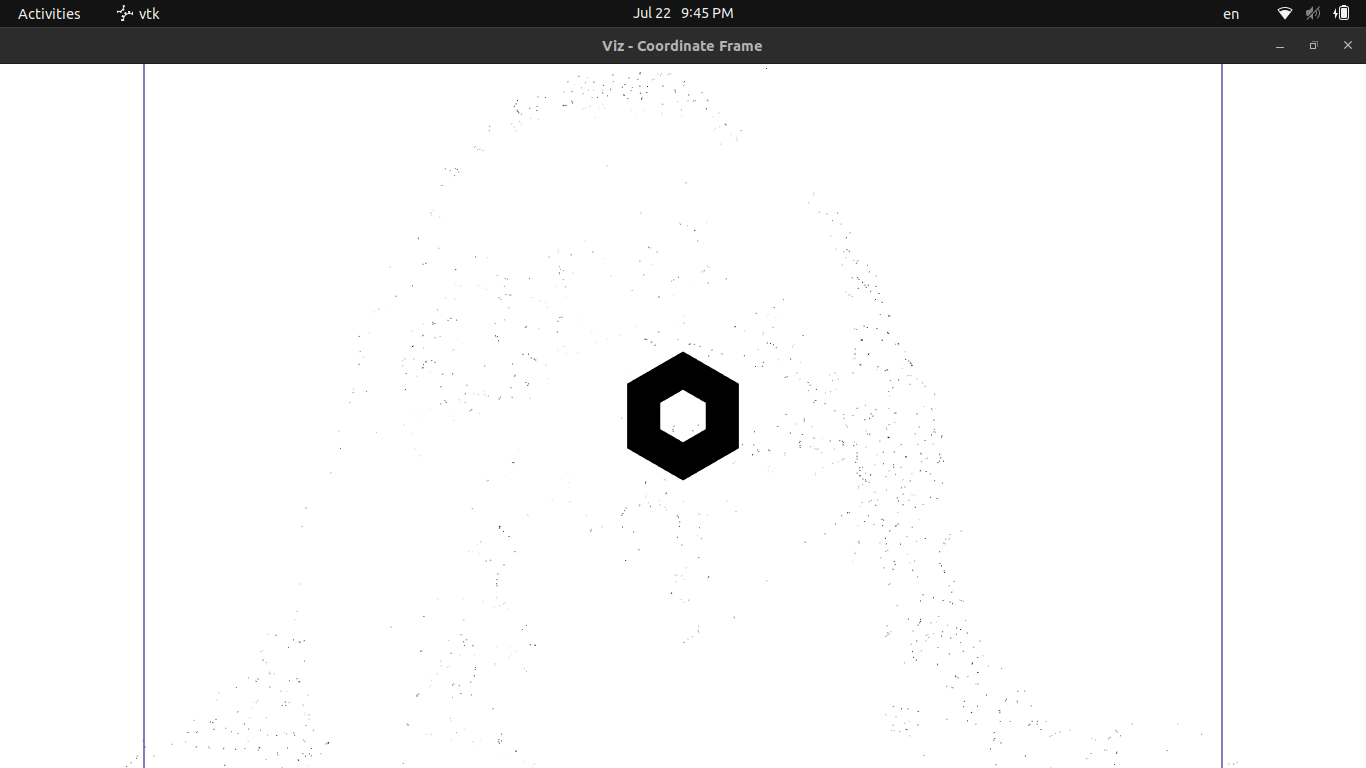
\includegraphics[scale=0.25]{images/opencv_sfm01.png}
	\end{figure}


	\begin{figure}
		\caption{Viewer}
		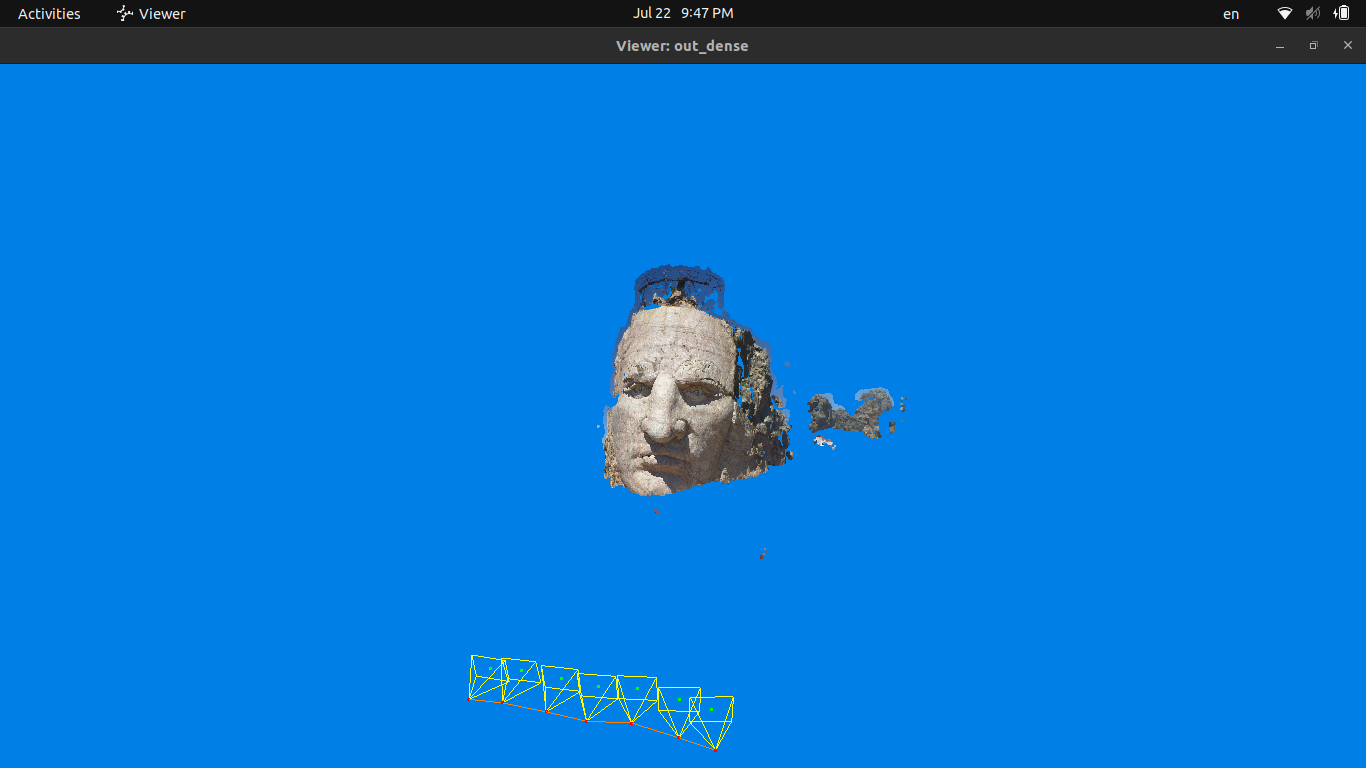
\includegraphics[scale=0.25]{images/opencv_sfm02.png}
	\end{figure}

	\begin{lstlisting}
// main.cpp
#define CERES_FOUND true
#define _USE_OPENCV true
#define OPENCV_TRAITS_ENABLE_DEPRECATED

#include <iostream>
#include <algorithm>
#include <string>
#include <numeric>

#include <opencv2/opencv.hpp>
#include <opencv2/sfm.hpp>
#include <opencv2/viz.hpp>
#include <opencv2/calib3d.hpp>
#include <opencv2/core.hpp>
#include <opencv2/core/utils/logger.hpp>
#include <opencv2/core/utils/filesystem.hpp>
#include <opencv2/xfeatures2d.hpp>

#include <boost/filesystem.hpp>
#include <boost/graph/graph_traits.hpp>
#include <boost/graph/adjacency_list.hpp>
#include <boost/graph/connected_components.hpp>
#include <boost/graph/graphviz.hpp>

#include <OpenMVS/MVS/Interface.h>

using namespace cv;
using namespace std;
namespace fs = boost::filesystem;


class StructureFromMotion {

public:
    StructureFromMotion(const string& dir,
                        const float matchSurvivalRate = 0.5f,
                        const bool viz = false,
                        const string mvs = "",
                        const string cloud = "",
                        const bool saveDebug = false)
            : PAIR_MATCH_SURVIVAL_RATE(matchSurvivalRate)
            , visualize(viz)
            , saveMVS(mvs)
            , saveCloud(cloud)
            , saveDebugVisualizations(saveDebug)

    {
        findImagesInDiretcory(dir);
    }

    void runSfM()
    {
        extractFeatures();
        matchFeatures();
        buildTracks();
        reconstructFromTracks();
        if (visualize) {
            visualize3D();
        }
        if (saveMVS != "") {
            saveToMVSFile();
        }
        if (saveCloud != "") {
//            CV_LOG_INFO(TAG, "Save point cloud to: " + saveCloud);
            viz::writeCloud(saveCloud, pointCloud, pointCloudColor);
        }
    }

private:
    void findImagesInDiretcory(const string& dir)
    {
//        CV_LOG_INFO(TAG, "Finding images in " + dir);

        utils::fs::glob(dir, "*.jpg", imagesFilenames);
        utils::fs::glob(dir, "*.JPG", imagesFilenames);
        utils::fs::glob(dir, "*.png", imagesFilenames);
        utils::fs::glob(dir, "*.PNG", imagesFilenames);

        std::sort(imagesFilenames.begin(), imagesFilenames.end());

//        CV_LOG_INFO(TAG, "Found " + std::to_string(imagesFilenames.size()) + " images");

//        CV_LOG_INFO(TAG, "Reading images...");
        for (const auto& i : imagesFilenames) {
//            CV_LOG_INFO(TAG, i);
            images[i] = imread(i);
            imageIDs[i] = images.size() - 1;
        }
    }

    void extractFeatures()
    {
//        CV_LOG_INFO(TAG, "Extract Features");

        auto detector = AKAZE::create();
        auto extractor = AKAZE::create();

        for (const auto& i : imagesFilenames) {
            Mat grayscale;
            cvtColor(images[i], grayscale, COLOR_BGR2GRAY);
            detector->detect(grayscale, keypoints[i]);
            extractor->compute(grayscale, keypoints[i], descriptors[i]);

//            CV_LOG_INFO(TAG, "Found " + to_string(keypoints[i].size()) + " keypoints in " + i);

            if (saveDebugVisualizations) {
                Mat out;
                drawKeypoints(images[i], keypoints[i], out, Scalar(0, 0, 255));
                imwrite(fs::basename(fs::path(i)) + "_features.jpg", out);
            }
        }
    }

    vector<DMatch> matchWithRatioTest(
            const DescriptorMatcher& matcher, const Mat& desc1, const Mat& desc2)
    {
        // Raw match
        vector<vector<DMatch>> nnMatch;
        matcher.knnMatch(desc1, desc2, nnMatch, 2);

        // Ratio test filter
        vector<DMatch> ratioMatched;
        for (size_t i = 0; i < nnMatch.size(); i++) {
            DMatch first = nnMatch[i][0];
            float dist1 = nnMatch[i][0].distance;
            float dist2 = nnMatch[i][1].distance;

            if (dist1 < MATCH_RATIO_THRESHOLD * dist2) {
                ratioMatched.push_back(first);
            }
        }

        return ratioMatched;
    }

    void matchFeatures()
    {
//        CV_LOG_INFO(TAG, "Match Features");

        BFMatcher matcher(NORM_HAMMING);

        for (size_t i = 0; i < imagesFilenames.size() - 1; ++i) {
            for (size_t j = i + 1; j < imagesFilenames.size(); ++j) {
                const string imgi = imagesFilenames[i];
                const string imgj = imagesFilenames[j];

                // Match with ratio test filter
                vector<DMatch> match
                        = matchWithRatioTest(matcher, descriptors[imgi], descriptors[imgj]);

                // Reciprocity test filter
                vector<DMatch> matchRcp
                        = matchWithRatioTest(matcher, descriptors[imgj], descriptors[imgi]);
                vector<DMatch> merged;
                for (const DMatch& dmr : matchRcp) {
                    bool found = false;
                    for (const DMatch& dm : match) {
                        // Only accept match if 1 matches 2 AND 2 matches 1.
                        if (dmr.queryIdx == dm.trainIdx and dmr.trainIdx == dm.queryIdx) {
                            merged.push_back(dm);
                            found = true;
                            break;
                        }
                    }
                    if (found) {
                        continue;
                    }
                }

                // Fundamental matrix filter
                vector<uint8_t> inliersMask(merged.size());
                vector<Point2f> imgiPoints, imgjPoints;
                for (const auto& m : merged) {
                    imgiPoints.push_back(keypoints[imgi][m.queryIdx].pt);
                    imgjPoints.push_back(keypoints[imgj][m.trainIdx].pt);
                }
                findFundamentalMat(imgiPoints, imgjPoints, inliersMask);

                vector<DMatch> final;
                for (size_t m = 0; m < merged.size(); m++) {
                    if (inliersMask[m]) {
                        final.push_back(merged[m]);
                    }
                }

                if ((float) final.size() / (float)match.size() < PAIR_MATCH_SURVIVAL_RATE) {
//                    CV_LOG_INFO(TAG,
//                                "Final match '" + imgi + "'->'" + imgj + "' has less than "
//                                + to_string(PAIR_MATCH_SURVIVAL_RATE) + " inliers from orignal. Skip");
                    continue;
                }

                matches[make_pair(imgi, imgj)] = final;

//                CV_LOG_INFO(TAG,
//                            "Matching " + imgi + " and " + imgj + ": " + to_string(final.size()) + " / "
//                            + to_string(match.size()));

                if (saveDebugVisualizations) {
                    Mat out;
                    vector<DMatch> rawmatch;
                    matcher.match(descriptors[imgi], descriptors[imgj], rawmatch);
                    vector<pair<string, vector<DMatch>&>> showList { { "Raw Match", rawmatch },
                                                                     { "Ratio Test Filter", match }, { "Reciprocal Filter", merged },
                                                                     { "Epipolar Filter", final } };
                    for (size_t i = 0; i < showList.size(); i++) {
                        drawMatches(images[imgi], keypoints[imgi], images[imgj], keypoints[imgj],
                                    showList[i].second, out, CV_RGB(255, 0, 0));
                        cv::putText(out, showList[i].first, Point(10, 50), FONT_HERSHEY_COMPLEX, 2.0,
                                    CV_RGB(255, 255, 255), 2);
                        cv::putText(out, "# Matches: " + to_string(showList[i].second.size()),
                                    Point(10, 100), FONT_HERSHEY_COMPLEX, 1.0, CV_RGB(255, 255, 255));
                        cv::imwrite(fs::basename(fs::path(imgi)) + "_" + fs::basename(fs::path(imgj))
                                    + "_" + to_string(i) + ".jpg",
                                    out);
                    }
                }
            }
        }
    }

    void buildTracks()
    {
//        CV_LOG_INFO(TAG, "Build tracks");

        using namespace boost;

        struct ImageFeature {
            string image;
            size_t featureID;
        };
        typedef adjacency_list<listS, vecS, undirectedS, ImageFeature> Graph;
        typedef graph_traits<Graph>::vertex_descriptor Vertex;

        map<pair<string, int>, Vertex> vertexByImageFeature;

        Graph g;

        // Add vertices - image features
        for (const auto& imgi : keypoints) {
            for (size_t i = 0; i < imgi.second.size(); i++) {
                Vertex v = add_vertex(g);
                g[v].image = imgi.first;
                g[v].featureID = i;
                vertexByImageFeature[make_pair(imgi.first, i)] = v;
            }
        }

        // Add edges - feature matches
        for (const auto& match : matches) {
            for (const DMatch& dm : match.second) {
                Vertex& vI = vertexByImageFeature[make_pair(match.first.first, dm.queryIdx)];
                Vertex& vJ = vertexByImageFeature[make_pair(match.first.second, dm.trainIdx)];
                add_edge(vI, vJ, g);
            }
        }

        using Filtered = filtered_graph<Graph, keep_all, std::function<bool(Vertex)>>;
        Filtered gFiltered(g, keep_all {}, [&g](Vertex vd) { return degree(vd, g) > 0; });

        // Get connected components
        std::vector<int> component(num_vertices(gFiltered), -1);
        int num = connected_components(gFiltered, &component[0]);
        map<int, vector<Vertex>> components;
        for (size_t i = 0; i != component.size(); ++i) {
            if (component[i] >= 0) {
                components[component[i]].push_back(i);
            }
        }
        // Filter bad components (with more than 1 feature from a single image)
        std::vector<int> vertexInGoodComponent(num_vertices(gFiltered), -1);
        map<int, vector<Vertex>> goodComponents;
        for (const auto& c : components) {
            set<string> imagesInComponent;
            bool isComponentGood = true;
            for (int j = 0; j < c.second.size(); ++j) {
                const string imgId = g[c.second[j]].image;
                if (imagesInComponent.count(imgId) > 0) {
                    // Image already represented in this component
                    isComponentGood = false;
                    break;
                } else {
                    imagesInComponent.insert(imgId);
                }
            }
            if (isComponentGood) {
                for (int j = 0; j < c.second.size(); ++j) {
                    vertexInGoodComponent[c.second[j]] = 1;
                }
                goodComponents[c.first] = c.second;
            }
        }

        Filtered gGoodComponents(g, keep_all {},
                                 [&vertexInGoodComponent](Vertex vd) { return vertexInGoodComponent[vd] > 0; });

//        CV_LOG_INFO(TAG, "Total number of components found: " + to_string(components.size()));
//        CV_LOG_INFO(TAG, "Number of good components: " + to_string(goodComponents.size()));
        const int accum = std::accumulate(goodComponents.begin(), goodComponents.end(), 0,
                                          [](int a, pair<const int, vector<Vertex>>& v) { return a + v.second.size(); });
//        CV_LOG_INFO(TAG,
//                    "Average component size: " + to_string((float)accum / (float)(goodComponents.size())));

        if (saveDebugVisualizations) {
            struct my_node_writer {
                my_node_writer(Graph& g_, const map<string, int>& iid_)
                        : g(g_)
                        , iid(iid_) {};
                void operator()(std::ostream& out, Vertex v)
                {
                    const int imgId = iid[g[v].image];
                    out << " [label=\"" << imgId
                        << "\" colorscheme=\"accent8\" fillcolor=" << (imgId + 1)
                        << " style=filled]";
                };
                Graph g;
                map<string, int> iid;
            };
            std::ofstream ofs("match_graph_good_components.dot");
            write_graphviz(ofs, gGoodComponents, my_node_writer(g, imageIDs));
            std::ofstream ofsf("match_graph_filtered.dot");
            write_graphviz(ofsf, gFiltered, my_node_writer(g, imageIDs));
        }

        // Each component is a track
        const size_t nViews = imagesFilenames.size();
        tracks.resize(nViews);
        for (int i = 0; i < nViews; i++) {
            tracks[i].create(2, goodComponents.size(), CV_64FC1);
            tracks[i].setTo(-1.0);
        }
        int i = 0;
        for (auto c = goodComponents.begin(); c != goodComponents.end(); ++c, ++i) {
            for (const int v : c->second) {
                const int imageID = imageIDs[g[v].image];
                const size_t featureID = g[v].featureID;
                const Point2f p = keypoints[g[v].image][featureID].pt;
                tracks[imageID].at<double>(0, i) = p.x;
                tracks[imageID].at<double>(1, i) = p.y;
            }
        }

        if (saveDebugVisualizations) {
            vector<Scalar> colors
                    = { CV_RGB(240, 248, 255), CV_RGB(250, 235, 215), CV_RGB(0, 255, 255),
                        CV_RGB(127, 255, 212), CV_RGB(240, 255, 255), CV_RGB(245, 245, 220),
                        CV_RGB(255, 228, 196), CV_RGB(255, 235, 205), CV_RGB(0, 0, 255),
                        CV_RGB(138, 43, 226), CV_RGB(165, 42, 42), CV_RGB(222, 184, 135) };

            vector<Mat> imagesM;
            for (const auto m : images)
                imagesM.push_back(m.second);
            Mat out;
            hconcat(vector<Mat>(imagesM.begin(), imagesM.begin() + 4), out);
            RNG& rng = cv::theRNG();
            const Size imgS = imagesM[0].size();
            for (int tId = 0; tId < 20; tId++) {
                const int trackId = rng(tracks[0].cols); // Randomize a track ID

                // Show track over images
                for (int i = 0; i < 3; i++) {
                    Point2f a = Point2f(tracks[i].col(trackId));
                    Point2f b = Point2f(tracks[i + 1].col(trackId));

                    if (a.x < 0 or a.y < 0 or b.x < 0 or b.y < 0) {
                        continue;
                    }

                    const Scalar c = colors[tId % colors.size()];
                    a.x += imgS.width * i;
                    b.x += imgS.width * (i + 1);
                    circle(out, a, 7, c, FILLED);
                    circle(out, b, 7, c, FILLED);
                    line(out, a, b, c, 3);
                }
                cv::imwrite("tracks.jpg", out);

                // Show track patches
                const int patchSize = 20;
                const Point2f patch(patchSize, patchSize);
                for (int i = 0; i < tracks.size(); i++) {
                    Point2f a = Point2f(tracks[i].col(trackId));
                    if (a.x < patchSize or a.y < patchSize or a.x > imgS.width - patchSize
                        or a.y > imgS.height - patchSize) {
                        continue;
                    }

                    cv::imwrite("track_" + to_string(trackId) + "_" + to_string(i) + ".png",
                                imagesM[i](Rect(a - patch, a + patch)));
                }
            }
        }
    }

    bool reconstructFromTracks()
    {
//        CV_LOG_INFO(TAG, "Reconstruct from " + to_string(tracks[0].cols) + " tracks");
        const Size imgS = images.begin()->second.size();
        const float f = std::max(imgS.width, imgS.height);
        Mat K
                = Mat(Matx33f { f, 0.0, imgS.width / 2.0f, 0.0, f, imgS.height / 2.0f, 0.0, 0.0, 1.0 });
        cv::sfm::reconstruct(tracks, Rs, Ts, K, points3d, true);

        K.copyTo(K_);

//        CV_LOG_INFO(TAG, "Reconstruction: ");
//        CV_LOG_INFO(TAG, "Estimated 3D points: " + to_string(points3d.size()));
//        CV_LOG_INFO(TAG, "Estimated cameras: " + to_string(Rs.size()));
//        CV_LOG_INFO(TAG, "Refined intrinsics: ");
//        CV_LOG_INFO(TAG, K_);

        if (Rs.size() != imagesFilenames.size()) {
//            CV_LOG_ERROR(TAG,
//                         "Unable to reconstruct all camera views (" + to_string(imagesFilenames.size())
//                         + ")");
            return false;
        }

        if (tracks[0].cols != points3d.size()) {
//            CV_LOG_WARNING(
//                    TAG, "Unable to reconstruct all tracks (" + to_string(tracks[0].cols) + ")");
        }

        // Create the point cloud
        pointCloud.clear();
        for (const auto& p : points3d)
            pointCloud.emplace_back(Vec3f(p));

        // Get the point colors
        pointCloudColor.resize(pointCloud.size(), Vec3b(0, 255, 0));
        vector<Point2f> point2d(1);
        for (int i = 0; i < (int)pointCloud.size(); i++) {
            for (int j = 0; j < imagesFilenames.size(); ++j) {
                Mat point3d = Mat(pointCloud[i]).reshape(1, 1);
                cv::projectPoints(point3d, Rs[j], Ts[j], K_, Mat(), point2d);
                if (point2d[0].x < 0 or point2d[0].x >= imgS.width or point2d[0].y < 0
                    or point2d[0].y >= imgS.height) {
                    continue;
                }
                pointCloudColor[i] = images[imagesFilenames[j]].at<Vec3b>(point2d[0]);
                break;
            }
        }

        return true;
    }

    void visualize3D()
    {
//        CV_LOG_INFO(TAG, "Visualize reconstruction");

        if (saveDebugVisualizations) {
            // 3d point reprojections
            Mat points2d;
            Mat points3dM(points3d.size(), 1, CV_32FC3);
            for (int i = 0; i < points3d.size(); i++) {
                points3dM.at<Vec3f>(i) = Vec3f(points3d[i]);
            }
            for (int j = 0; j < imagesFilenames.size(); j++) {
                cv::projectPoints(points3dM, Rs[j], Ts[j], K_, noArray(), points2d);

                Mat out;
                images[imagesFilenames[j]].copyTo(out);
                for (int i = 0; i < points2d.rows; i++) {
                    circle(out, points2d.at<Point2f>(i), 3, CV_RGB(255, 0, 0), FILLED);
                }
                cv::imwrite("reprojection_" + to_string(j) + ".jpg", out);
            }
        }

        // Create 3D windows
        viz::Viz3d window("Coordinate Frame");
        window.setWindowSize(Size(500, 500));
        window.setWindowPosition(Point(150, 150));
        window.setBackgroundColor(viz::Color::white());

        // Recovering cameras
        vector<Affine3d> path;
        for (size_t i = 0; i < Rs.size(); ++i)
            path.push_back(Affine3d(Rs[i], Ts[i]));

        // Add the pointcloud
        viz::WCloud cloud_widget(pointCloud, pointCloudColor);
        window.showWidget("point_cloud", cloud_widget);
        // Add cameras
        window.showWidget("cameras_frames_and_lines",
                          viz::WTrajectory(path, viz::WTrajectory::BOTH, 0.1, viz::Color::black()));
        window.showWidget(
                "cameras_frustums", viz::WTrajectoryFrustums(path, K_, 0.1, viz::Color::navy()));
        window.setViewerPose(path[0]);

        /// Wait for key 'q' to close the window
//        CV_LOG_INFO(TAG, "Press 'q' to close ... ")

        window.spin();
    }

    void saveToMVSFile()
    {
//        CV_LOG_INFO(TAG, "Save reconstruction to MVS file: " + saveMVS)

        MVS::Interface interface;
        MVS::Interface::Platform p;

        // Add camera
        MVS::Interface::Platform::Camera c;
        const Size imgS = images[imagesFilenames[0]].size();
        c.K = Matx33d(K_);
        c.R = Matx33d::eye();
        c.C = Point3d(0, 0, 0);
        c.name = "Camera1";
        c.width = imgS.width;
        c.height = imgS.height;
        p.cameras.push_back(c);

        // Add views
        p.poses.resize(Rs.size());
        for (size_t i = 0; i < Rs.size(); ++i) {
            Mat t = -Rs[i].t() * Ts[i];
            p.poses[i].C.x = t.at<double>(0);
            p.poses[i].C.y = t.at<double>(1);
            p.poses[i].C.z = t.at<double>(2);
            Mat r;
            Rs[i].copyTo(r);
            Mat(r).convertTo(p.poses[i].R, CV_64FC1);

            // Add corresponding image
            MVS::Interface::Image image;
            image.cameraID = 0;
            image.poseID = i;
            image.name = imagesFilenames[i];
            image.platformID = 0;
            interface.images.push_back(image);
        }
        p.name = "Platform1";
        interface.platforms.push_back(p);

        // Add point cloud
        for (size_t k = 0; k < points3d.size(); ++k) {
            MVS::Interface::Color c;
            MVS::Interface::Vertex v;
            v.X = Vec3f(points3d[k]);

            // Reproject to see if in image bounds and get the RGB color
            Mat point3d;
            Mat(points3d[k].t()).convertTo(point3d, CV_32FC1);
            for (uint32_t j = 0; j < tracks.size(); ++j) {
                vector<Point2f> points2d(1);
                cv::projectPoints(point3d, Rs[j], Ts[j], K_, Mat(), points2d);
                if (points2d[0].x < 0 or points2d[0].x > imgS.width or points2d[0].y < 0
                    or points2d[0].y > imgS.height) {
                    continue;
                } else {
                    c.c = images[imagesFilenames[j]].at<Vec3b>(points2d[0]);
                    v.views.push_back({ j, 1.0 });
                }
            }

            interface.verticesColor.push_back(c);
            interface.vertices.push_back(v);
        }

        MVS::ARCHIVE::SerializeSave(interface, saveMVS);
    }

    vector<String> imagesFilenames;
    map<string, int> imageIDs;
    map<string, Mat> images;
    map<string, vector<KeyPoint>> keypoints;
    map<string, Mat> descriptors;
    map<pair<string, string>, vector<DMatch>> matches;
    vector<Mat> Rs, Ts;
    vector<Mat> points3d;
    vector<Mat> tracks;
    vector<Vec3f> pointCloud;
    vector<Vec3b> pointCloudColor;
    Matx33f K_;

    const float MATCH_RATIO_THRESHOLD = 0.8f; // Nearest neighbor matching ratio
    const float
            PAIR_MATCH_SURVIVAL_RATE; // Ratio of surviving matches for a successful stereo match
    const bool visualize; // Show 3D visualization of the sprase cloud?
    const string saveMVS; // Save the reconstruction in MVS format for OpenMVS?
    const string saveCloud; // Save the reconstruction to a point cloud file?
    const bool saveDebugVisualizations; // Save debug visualizations from the reconstruction process

    const string TAG = "StructureFromMotion";
};

int main(int argc, char** argv)
{
    utils::logging::setLogLevel(utils::logging::LOG_LEVEL_DEBUG);

    cv::CommandLineParser parser(argc, argv,
                                 "{help h ? |       | help message}"
                                 "{@dir     | .     | directory with image files for reconstruction }"
                                 "{mrate    | 0.5   | Survival rate of matches to consider image pair success }"
                                 "{viz      | false | Visualize the sparse point cloud reconstruction? }"
                                 "{debug    | false | Save debug visualizations to files? }"
                                 "{mvs      |       | Save reconstruction to an .mvs file. Provide filename }"
                                 "{cloud    |       | Save reconstruction to a point cloud file (PLY, XYZ and OBJ). Provide "
                                 "filename}");

    if (parser.has("help")) {
        parser.printMessage();
        return 0;
    }

    StructureFromMotion sfm(parser.get<string>("@dir"), parser.get<float>("mrate"),
                            parser.get<bool>("viz"), parser.get<string>("mvs"), parser.get<string>("cloud"),
                            parser.get<bool>("debug"));
    sfm.runSfM();

    return 0;
}

	\end{lstlisting}

	\begin{lstlisting}
// CMakeList.txt		
cmake_minimum_required(VERSION 3.22)
project(sfm)

set(CMAKE_CXX_STANDARD 14)
set(CMAKE_CXX_STANDARD_REQUIRED ON)
set(CMAKE_BUILD_TYPE Release)

add_executable(sfm main.cpp)

find_package(Ceres QUIET)

set(OpenCV_DIR "" CACHE PATH "/mnt/ntfs/Data/code/CV/source/opencv/build")
find_package(OpenCV 4.5.5 REQUIRED COMPONENTS core calib3d features2d sfm viz)

find_package(Eigen3 REQUIRED)

set(OpenMVS_DIR "" CACHE PATH "/mnt/ntfs/Data/code/CV/source/openMVS/build")
find_package(OpenMVS REQUIRED)

find_package(Boost REQUIRED COMPONENTS filesystem graph)

include_directories(${EIGEN3_INCLUDE_DIR} ${OpenMVS_INCLUDE_DIRS} ${Boost_INCLUDE_DIR})

message(STATUS ${OpenCV_LIBRARIES} ${OpenMVS_LIBRARIES})

target_link_libraries(sfm
        ${OpenCV_LIBRARIES}
        ${Boost_LIBRARIES}
#        ${OpenMVS_LIBRARIES}
        )

	\end{lstlisting}
\end{document}